\subsection{Controller and Plant Testing}
\label{sec:pwrtesting}

{\bf \color{red} This section is not finished - I need to finish my analysis.}
\subsubsection{Plant Tests}

Step responses were observed for the components, these conformed to expectations and the test was deemed successful.
{\color{red}Step Response Figures Here}

Tanks were tested and operated as expected.


\subsubsection{Plant with a PID/PD Combination}

I found that the system was able to give a good response.
Response was not optimal, and there were issues with the Electrolyser {\color{red}(comment more)}

\subsubsection{Plant with LQR Controller}

\subsubsection{Plant with a Augmented LQR Combination}
\begin{figure}[htp]
\centering
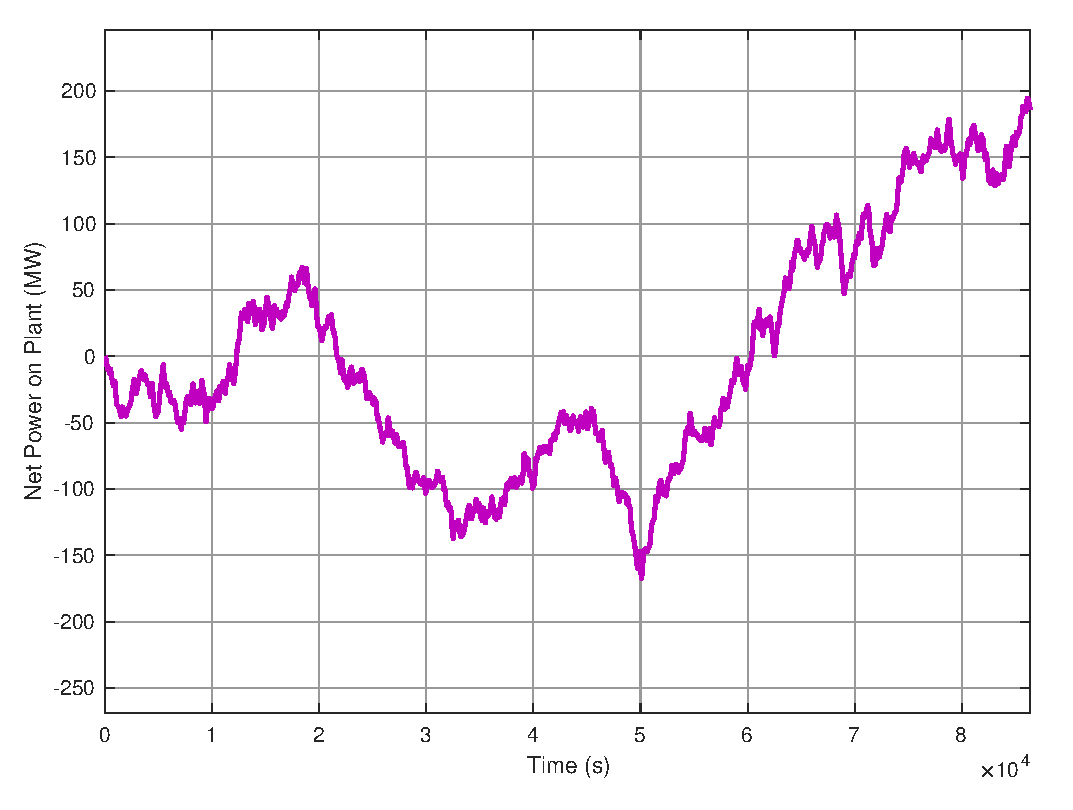
\includegraphics[width=.33\textwidth]{images/sim/sim1_disturb.eps}\hfill
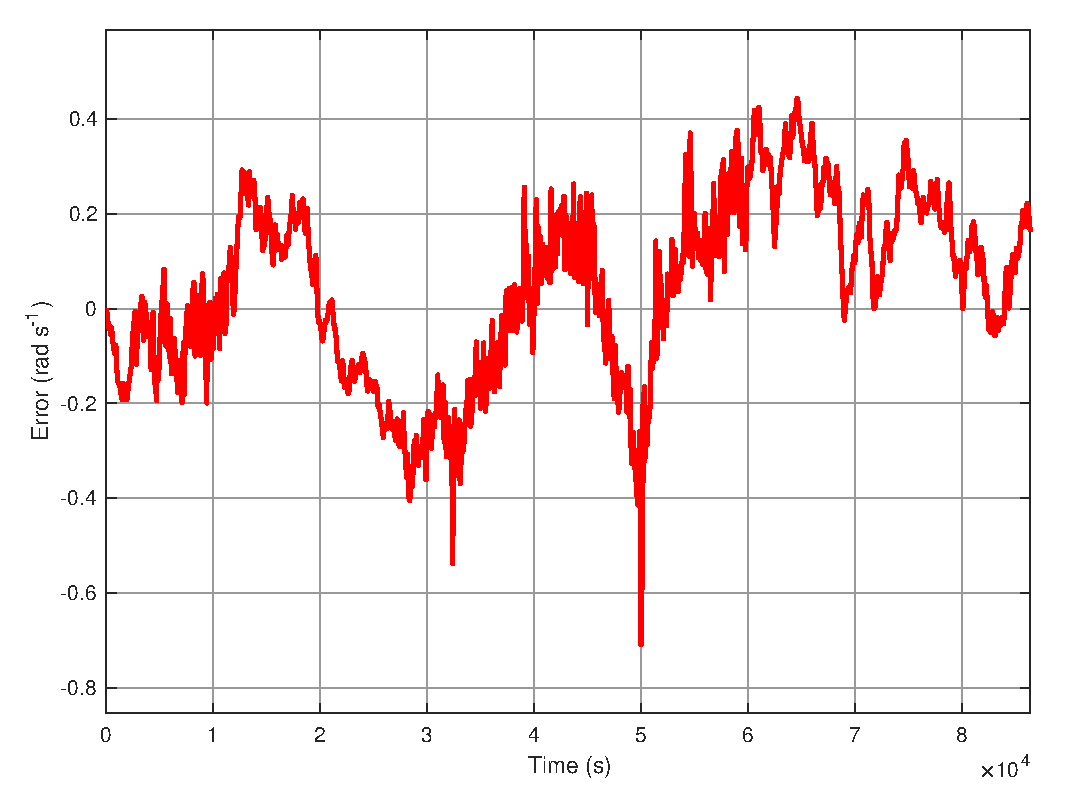
\includegraphics[width=.33\textwidth]{images/sim/sim1_omega.eps}\hfill
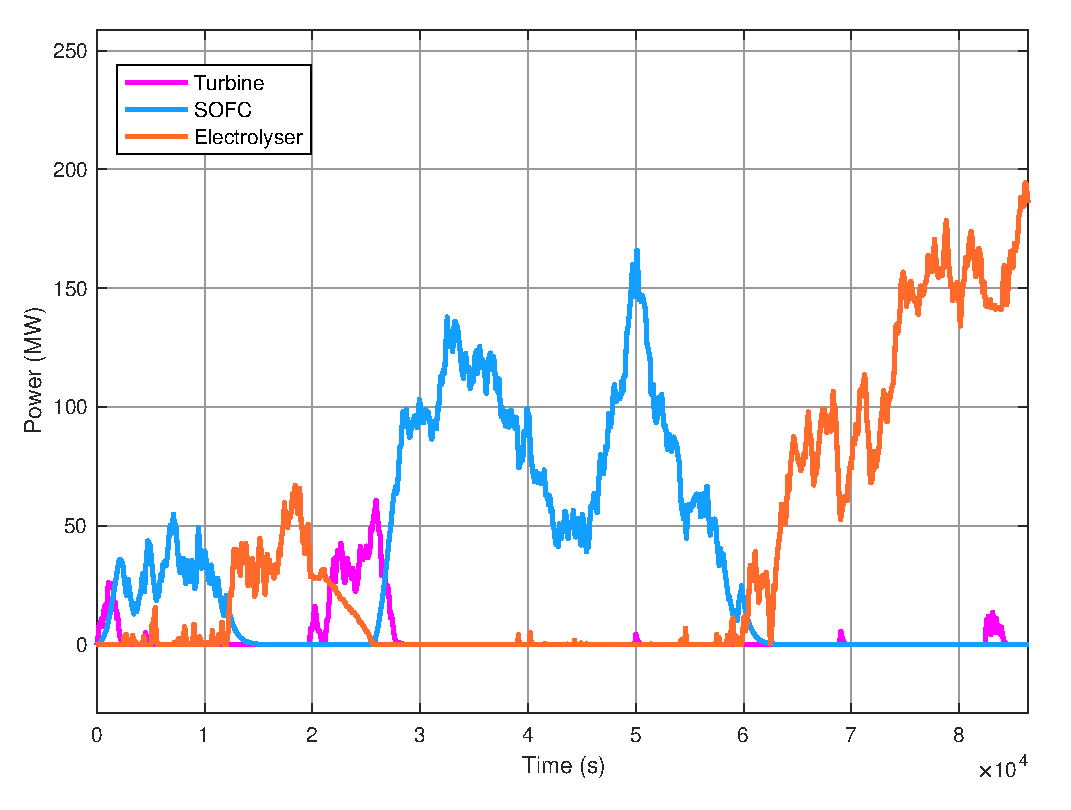
\includegraphics[width=.33\textwidth]{images/sim/sim1_util.eps}
        \caption{Simulation Run for LQR Controller with Augmented States, under \emph{Very Harsh} Conditions To Demonstrate Controller Robustness.}
        \label{fig:sim1}
\end{figure}
System was able to perform well under simulated harsh conditions, with minimal frequency error under a low inertia state.

Compared to PID I observed step responses are {\color{red}XXXX}.
%%todo make this better

\begin{itemize}
{\color{red}
\item We need to model errors in the system we predict
\item We need to model errors in efficiency assumptions - check with less efficient systems
\item We need to model errors in disturbance prediction - see above
}
\end{itemize}
